\section{Evaluation}
\label{sec:results}

Next, we describe the data we used to train the models required to extract the features, the training of the classifier, and the results of our submission.

\subsection{Computation of features}

We need to generate two types of models to extract our features: probabilistic lexicons and language models. We used the probabilistic lexicons that can be obtained as a sub product of the training of full statistical models. In particular, we used Moses~\cite{Moses} on its default configuration with the News Commentary V13 parallel corpus as provided for the News translation shared task. We used the same corpora to train the language models. In this case, we used Kenlm~\cite{Kenlm} and estimated models of order $5$.


\subsection{Training the classifier}

We trained the classifier using again the News Commentary parallel corpus. We generate as many negative examples as positive sentence pairs in the corpus for a total of almost $600$k data points to train our classifier. The negative examples were evenly distributed among the thee perturbation operations described in the previous section. We used scikit-learn to train our gradient boosting classifier. The final trained model is used to score all sentences in the noisy corpus.

We perform some initial experiments using the Common Crawl corpus, under the rationale that it would be closer to the domain of the noisy data belonging to the Paracrawl corpus. However, Common Crawl data has quite a large number of misaligned sentences. This will result in positive data points that in reality were negative which will hinder the learning process of the classifier. We tried an iterative cleaning process so that we were not so reliant in clean, perfectly align data. However, we had to stop exploring this direction due to time constraints.


%https://docs.google.com/spreadsheets/d/1SKMOBbH5YVsQJpbUCMN3K8Gzt_89zBabQl716Aw8NjM/edit?usp=sharing
\begin{figure}[ht]
  \centering
  \begin{subfigure}[b]{\columnwidth}
    \hspace*{-1.5em}
    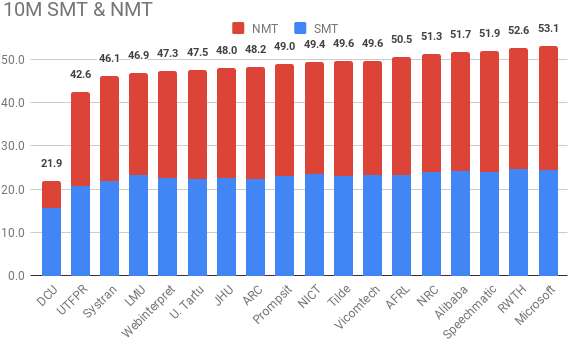
\includegraphics[width=1.1\textwidth]{images/10M_crop.png}
    \label{fig:10M}
  \end{subfigure}
  ~
  \begin{subfigure}[b]{\columnwidth}
    \hspace*{-1.5em}
    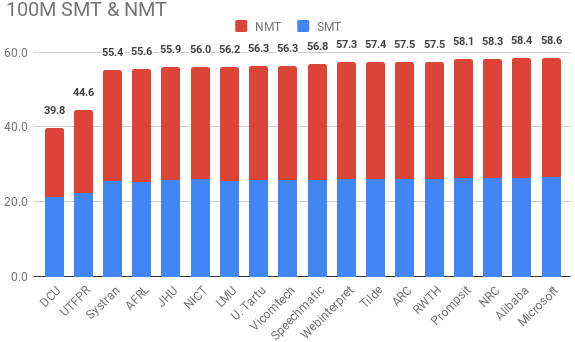
\includegraphics[width=1.1\textwidth]{images/100M_crop.png}
    \label{fig:100M}
  \end{subfigure}
  \caption{Best submission of each participant institution. We display BLEU [\%] results stacked for SMT (\textcolor{blue}{blue}) and NMT (\textcolor{red}{red}).}
  \label{fig:results}
\end{figure}

\subsection{Results}

Participants in the shared task have to submit a file with quality scores, one per line, corresponding to the sentence pairs on the 1 billion word German–English Paracrawl corpus. Scores do not have to be meaningful, except that higher scores indicate better quality. Evaluation of the quality scores is done by sub-sampling $10$ million and $100$ million word corpora based on these scores, training statistical~\cite{Moses} and neural~\cite{Marian} machine translation systems with these corpora, and evaluation translation quality on six blind test sets\footnote{Tests: newstest 2018, iwslt 2017, Acquis, EMEA, Global Voices, and KDE.} using the BLEU~\cite{Bleu} score. 

Figure~\ref{fig:results} displays the score of the best submission of each individual participant institution. Plot in top shows results for the $10$ million token sub-sampled corpus, while the top in the bottom shows results for the $100$ million token corpus. Scores are the aggregation of the BLEU scores of the statistical and neural systems averaged over the six blind test sets.

One first observation we can make is that (almost) all scores quite close to each other with little variation between them; specially in the $100$ million condition. Also, scores by the statistical and neural systems tend to follow the same pattern. We do not have confidence intervals available which makes difficult to interpret the observed differences between systems. Still, in the case of $100$ million tokens sub-sampling, it seems quite clear that all systems besides DCU and UTFPR are of the same quality. There is only a $5\%$ relative improvement between the last system of this group and the best submission to the task. Scores are a bit more spread out in the $10$ million tokens sub-sampling. This seems to indicate that $100$ million token is too large a number since it allows (almost) all systems to reach a theoretical maximum.

Our submission (MAJE) scored $47.3$ in the $10$ million tokens sub-sampling in comparison to the $53.1$ scored by the best submission. For the $100$ million condition, we scored $57.3$ in comparison to $58.6$ best score.